% -*- coding: utf-8 -*-
\documentclass[UTF8,a4paper,10pt]{ctexart}

\usepackage[left=3.17cm, right=3.17cm, top=2.74cm, bottom=2.74cm]{geometry}
\usepackage{amsmath}
\usepackage{amssymb}
\usepackage{graphicx,subfig}
\usepackage{float}
\usepackage{caption}
\usepackage{enumerate}
\usepackage{booktabs}
\usepackage{multirow}
\usepackage{array}
\usepackage{longtable}
\usepackage[colorlinks=true,linkcolor=black,citecolor=black,urlcolor=blue]{hyperref}
\usepackage{xcolor}
\usepackage{listings}
\usepackage{fancyhdr}
\usepackage{algorithm}
\usepackage{algorithmicx}
\usepackage{algpseudocode}
\usepackage{enumitem}
\usepackage{pifont}
\usepackage{tikz}
\usepackage{eso-pic}
\usepackage{framed}

\newcommand{\tabincell}[2]{\begin{tabular}{@{}#1@{}}#2\end{tabular}}

\newcommand{\yihao}{\fontsize{26pt}{36pt}\selectfont}
\newcommand{\erhao}{\fontsize{22pt}{28pt}\selectfont}
\newcommand{\xiaoer}{\fontsize{18pt}{18pt}\selectfont}
\newcommand{\sanhao}{\fontsize{16pt}{24pt}\selectfont}
\newcommand{\xiaosan}{\fontsize{15pt}{22pt}\selectfont}
\newcommand{\sihao}{\fontsize{14pt}{21pt}\selectfont}
\newcommand{\banxiaosi}{\fontsize{13pt}{19.5pt}\selectfont}
\newcommand{\xiaosi}{\fontsize{12pt}{18pt}\selectfont}
\newcommand{\dawuhao}{\fontsize{11pt}{11pt}\selectfont}
\newcommand{\wuhao}{\fontsize{10.5pt}{15.75pt}\selectfont}

\ctexset{
  section = {
    format = \bfseries\zihao{4},
    name = {,、},
    number = \chinese{section}
  },
  subsection = {
    format = \bfseries\zihao{-4},
    name = {（,）},
    number = \chinese{subsection}
  },
  subsubsection = {
    format = \bfseries\zihao{5},
    number = \arabic{subsubsection}
  }
}

\pagestyle{fancy}
\lhead{\kaishu 数据安全课程作业}
\chead{基于 Paillier 算法的隐私信息获取实验}
\rhead{祝铭堃 2312309}
\lfoot{}
\cfoot{\thepage}
\rfoot{}
\renewcommand{\headrulewidth}{0.1pt}
\renewcommand{\footrulewidth}{0pt}
\setlength{\headheight}{15pt}

\newcommand{\HRule}{\rule{\linewidth}{0.5mm}}
\newcommand{\HRulegrossa}{\rule{\linewidth}{1.2mm}}

\floatname{algorithm}{Algorithm}
\renewcommand{\algorithmicrequire}{\textbf{Input:}}
\renewcommand{\algorithmicensure}{\textbf{Output:}}

\lstset{
breaklines,
basicstyle=\small\ttfamily,
escapeinside=``,
keywordstyle=\color{blue!70}\bfseries,
commentstyle=\color{red!50!green!50!blue!50},
stringstyle=\ttfamily,
extendedchars=false,
linewidth=\textwidth,
numbers=left,
numberstyle=\tiny\color{blue!50},
frame=trbl,
rulesepcolor=\color{red!20!green!20!blue!20}
}

\newcommand{\cmark}{\ding{51}}
\newcommand{\xmark}{\ding{55}}
\newcommand{\done}{\rlap{$\square$}{\raisebox{2pt}{\large\hspace{1pt}\cmark}}\hspace{-2.5pt}}
\newcommand{\wontfix}{\rlap{$\square$}{\large\hspace{1pt}\xmark}}

\newcommand{\watermark}[3]{\AddToShipoutPictureBG{
\parbox[b][\paperheight]{\paperwidth}{
\vfill
\centering
\tikz[remember picture, overlay]
  \node [rotate = #1, scale = #2] at (current page.center)
    {\textcolor{gray!80!cyan!30!magenta!30}{#3}};
\vfill}}}

\newcommand{\screenshotplaceholder}[2]{
\begin{figure}[H]
    \centering
    \fbox{
    \begin{minipage}[c][5.0cm][c]{0.84\textwidth}
        \centering
        \textbf{#1}\\[0.8em]
        #2
    \end{minipage}}
    \caption{#1}
\end{figure}
}

\begin{document}
\renewcommand{\contentsname}{目录}
\renewcommand{\figurename}{图}
\renewcommand{\tablename}{表}
\renewcommand{\today}{\number\year 年 \number\month 月 \number\day 日}

\begin{titlepage}
    \begin{center}
    
\includegraphics[width=0.8\textwidth]{NKU.png}\\[1cm]
    \vspace{20mm}
    {\Huge \heiti 南开大学}\\[0.9cm]
    {\huge \heiti 网络空间安全学院}\\[0.9cm]
    {\Large \textbf{《数据安全》课程作业}}\\[0.8cm]
    \HRule \\[0.9cm]
    {\LARGE \bfseries 基于 Paillier 算法的隐私信息获取实验}\\[0.4cm]
    \HRule \\[2.0cm]
    \vspace{\fill}
    \centering
    {\LARGE 姓名\ :\ 祝铭堃}\\[0.5cm]
    {\LARGE 学号\ :\ 2312309}\\[0.5cm]
    {\LARGE 专业\ :\ 计算机科学与技术}\\[0.5cm]
    {\LARGE 指导教师\ :\ 刘哲理}\\[0.5cm]
    \vfill
    {\Large \today}
    \end{center}
\end{titlepage}

\newpage
\tableofcontents

\newpage
\watermark{60}{10}{NKU}
\setcounter{page}{1}

\section{实验要求}
\begin{enumerate}
    \item 基于 Paillier 算法实现隐私信息获取：从服务器给定的 $m$ 个消息中获取其中一个，不得向服务器泄露获取了哪一个消息，同时客户端能完成获取消息的解密。
    \item 扩展实验：客户端保存对称密钥 $k$，服务器端存储 $m$ 个用对称密钥 $k$ 加密的密文，通过隐私信息获取方法得到指定密文后能解密得到对应的明文。
\end{enumerate}

为便于后续实现和分析，我们在开始实验之前进一步明确了以下边界条件：
\begin{itemize}
    \item 威胁模型为单服务器、半诚实模型，服务器按协议执行，但会尝试根据收到的信息推断客户端的目标下标。
    \item 不考虑恶意客户端伪造查询、重放攻击与拒绝服务等主动攻击。
    \item 演示环境使用本机 \texttt{localhost} TCP 通信，保证“客户端/服务器”两端分离，同时便于复现实验。
\end{itemize}

\section{项目结构与仓库说明}
本次实验的代码、测试、结果数据以及报告源码均已整理在本地项目目录中，我们将核心内容组织如下：
\begin{itemize}
    \item \texttt{实验/lab1/pir\_lab/}：核心协议、编码、服务端、客户端实现
    \item \texttt{实验/lab1/scripts/}：运行入口、AES 密钥初始化脚本、基准测试脚本
    \item \texttt{实验/lab1/tests/}：自动化测试
    \item \texttt{实验/lab1/report/}：当前实验报告
\end{itemize}

本实验对应的 GitHub 仓库为 \href{https://github.com/EricEvans-e/data_security2026}{\texttt{EricEvans-e/data\_security2026}}。

当前报告对应的实验内容位于该仓库的 \texttt{实验/lab1/} 目录下，我们后续展示的代码、日志、测试结果与截图也都来自这一目录中的实际运行产物。

\section{实验原理}

\subsection{同态加密}
同态加密（Homomorphic Encryption, HE）是一类允许在密文上直接计算，并在解密后得到与明文上对应计算结果一致的密码机制。其核心价值在于：数据无需先解密就能被第三方处理，从而在计算过程中仍然保持隐私。

从运算能力看，同态加密通常分为以下几类：
\begin{itemize}
    \item \textbf{加法同态：} 若加密函数 $E$ 满足 $E(m_1)\times E(m_2)=E(m_1+m_2)$，则说明该方案支持加法同态。
    \item \textbf{乘法同态：} 若加密函数 $E$ 满足 $E(m_1)^n=E(m_1\times n)$，则说明该方案支持密文与明文常数之间的乘法同态。
    \item \textbf{全同态：} 若在一定条件下同时支持加法与乘法组合运算，则可在密文上完成更复杂的电路计算。
\end{itemize}

本实验所使用的 Paillier 方案属于加法同态方案，并支持“密文乘明文常数”的运算，因此非常适合构造 one-hot 选择向量式的 PIR。

\subsection{半同态加密}
半同态加密（Semi-Homomorphic Encryption）是同态加密的一个子类，只支持一种主要运算类型。本实验中的 Paillier 即属于半同态加密，它支持：
\begin{itemize}
    \item 密文与密文相乘，对应明文加法；
    \item 密文与明文常数相乘，对应明文标量乘法。
\end{itemize}

对两个明文 $m_1,m_2$ 而言，若对应密文分别为 $c_1=E(m_1)$、$c_2=E(m_2)$，则有：
\[
D(c_1 \cdot c_2)=m_1+m_2.
\]
对密文 $E(m)$ 与常数 $k$ 而言，则有：
\[
D(E(m)^k)=k \cdot m.
\]

正是由于具备这两个性质，服务器才能在不知道客户端目标下标的情况下，直接对加密选择向量与消息集合进行聚合计算。

\subsection{Paillier算法}
Paillier 公钥密码体制最早由 Pascal Paillier 于 1999 年提出。其主要过程如下：
\begin{enumerate}
    \item \textbf{密钥生成}
    \begin{itemize}
        \item 选取两个大素数 $p,q$；
        \item 计算 $n=pq$ 与 $\lambda=\mathrm{lcm}(p-1,q-1)$；
        \item 选择合适的 $g \in \mathbb{Z}_{n^2}^{*}$；
        \item 公钥为 $(n,g)$，私钥与 $\lambda$ 相关。
    \end{itemize}
    \item \textbf{加密}
    \begin{itemize}
        \item 对消息 $m \in \mathbb{Z}_n$，随机选择 $r \in \mathbb{Z}_n^*$；
        \item 计算
        \[
        c=g^m r^n \bmod n^2.
        \]
    \end{itemize}
    \item \textbf{解密}
    \begin{itemize}
        \item 通过
        \[
        m=\frac{L(c^\lambda \bmod n^2)}{L(g^\lambda \bmod n^2)} \bmod n
        \]
        恢复消息。
    \end{itemize}
    \item \textbf{加法同态验证}
    \begin{itemize}
        \item 若 $c_1=E(m_1)$、$c_2=E(m_2)$，则
        \[
        c_1c_2 \bmod n^2 = E(m_1+m_2).
        \]
    \end{itemize}
\end{enumerate}

在本实验中，Paillier 的使用方式并不是直接加密所有消息，而是用于加密客户端的选择向量，让服务器在不知下标的情况下完成同态聚合。

\section{实验过程}

\subsection{实验环境安装}

\subsubsection{安装Python环境}
本次实验在 Windows PowerShell 中完成。首先，我们切换到项目目录并激活 \texttt{datasec} 虚拟环境；然后，我们检查 Python 运行环境是否可以正常调用。实际实验中使用的是 Python 3.11.15，因此无需重新安装 Python，只需确认其版本与命令行调用均正常即可。从版本输出中，我们可以确认当前环境已经满足后续实验的基本要求。

\begin{lstlisting}[title=查看 Python 版本,frame=trbl,language={Python}]
python --version
\end{lstlisting}

这条命令用于确认当前终端能够正确调用 Python，同时也便于我们记录实验所使用的解释器版本。

\begin{figure}[H]
    \centering
    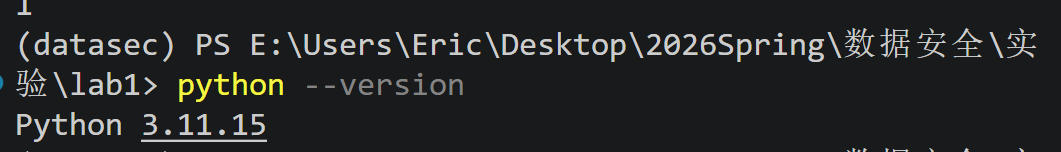
\includegraphics[width=0.88\textwidth]{../src/12.png}
    \caption{Python 运行环境检查结果}
\end{figure}

从图中可以看到，命令行提示符已经处于 \texttt{(datasec)} 虚拟环境中，随后系统正确返回 \texttt{Python 3.11.15}。这说明当前实验并不是调用系统中其他 Python 解释器，而是已经切换到了本实验专用环境。由于后续客户端、服务端、benchmark 与自动化测试都依赖同一套解释器与第三方库，因此先固定 Python 版本，可以减少因环境不一致导致的路径错误、包冲突或运行结果不稳定问题。

\subsubsection{安装phe库}
Paillier 的核心功能依赖 \texttt{phe} 库实现，因此我们先完成依赖安装：
\begin{lstlisting}[title=安装 phe 依赖,frame=trbl,language={Python}]
conda activate datasec
python -m pip install -r requirements.txt
\end{lstlisting}

这里我们直接通过 \texttt{requirements.txt} 统一安装依赖，这样可以保证客户端、服务端和测试脚本使用相同的软件环境。

实际安装完成后，我们确认 \texttt{phe}、\texttt{pycryptodome} 与 \texttt{pytest} 均已可以正常使用。这样，我们的基础依赖就准备好了。

\begin{figure}[H]
    \centering
    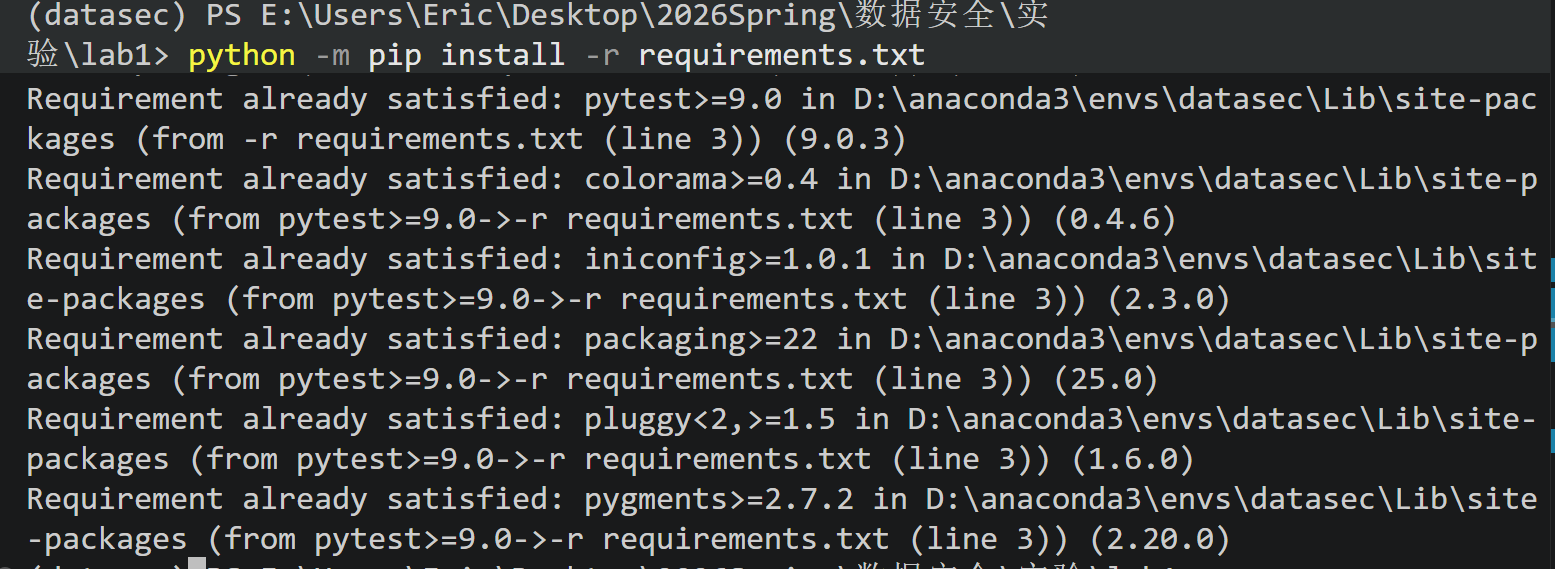
\includegraphics[width=0.95\textwidth]{../src/13.png}
    \caption{依赖安装与检查结果}
\end{figure}

结合安装截图可以看到，\texttt{python -m pip install -r requirements.txt} 执行后，终端依次给出了 \texttt{Requirement already satisfied} 的提示。这表明 \texttt{requirements.txt} 中列出的依赖已经存在于当前虚拟环境中，不需要重复下载即可直接使用。该文件中的核心依赖如下：
\begin{itemize}
    \item \texttt{phe==1.5.0}：用于实现 Paillier 加密与同态运算；
    \item \texttt{pycryptodome==3.23.0}：用于扩展实验中的 AES 加解密；
    \item \texttt{pytest>=9.0}：用于后续自动化测试。
\end{itemize}
统一由依赖文件管理还有一个好处，即报告中所有实验结果都可以在相同版本的软件栈上复现，从而增强实验过程的可重复性。

\subsubsection{验证环境正确性}
为了确认环境安装成功，我们继续执行导入验证：
\begin{lstlisting}[title=环境验证命令,frame=trbl,language={Python}]
python -c "from phe import paillier; from Crypto.Cipher import AES; print('ok')"
\end{lstlisting}

这条验证命令同时检查了 Paillier 库和 AES 库是否能够正常导入，因此足以作为最基本的环境连通性测试。

若输出 \texttt{ok}，说明依赖已经安装正确，我们就可以继续后续实验。这样，我们的 Python 环境检查也就完成了。

\begin{figure}[H]
    \centering
    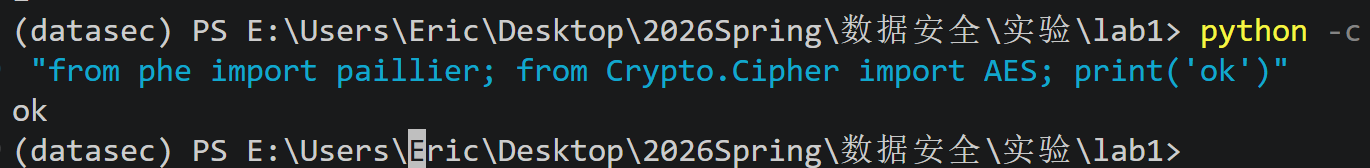
\includegraphics[width=0.92\textwidth]{../src/14.png}
    \caption{环境验证命令执行结果}
\end{figure}

从验证结果可以看到，命令执行后成功输出 \texttt{ok}，且没有出现模块未找到、导入失败或动态链接错误。这说明当前环境已经同时具备 Paillier 同态加密所需的 \texttt{phe} 模块，以及 AES 对称加密所需的 \texttt{Crypto.Cipher} 模块。换言之，当前 \texttt{lab1} 报告中涉及的基础 PIR 实现与扩展流程，都已经具备可运行的软件基础。完成这一步之后，我们后续展示的同态性质验证、客户端查询和 benchmark 数据才具有可信的环境前提。

\subsection{基于Python的phe库完成加法和标量乘法的验证}
在正式实现隐私信息获取之前，我们先验证 \texttt{phe} 库是否确实满足课程中涉及的加法同态与标量乘法性质。测试代码如下：
\begin{lstlisting}[title=同态运算验证代码,frame=trbl,language={Python}]
from phe import paillier
import time

print("默认私钥大小：", paillier.DEFAULT_KEYSIZE)
public_key, private_key = paillier.generate_paillier_keypair()
message_list = [3.1415926, 100, -4.6e-12]

time_start_enc = time.time()
encrypted_message_list = [public_key.encrypt(m) for m in message_list]
time_end_enc = time.time()
print("加密耗时(s)：", time_end_enc - time_start_enc)

time_start_dec = time.time()
decrypted_message_list = [private_key.decrypt(c) for c in encrypted_message_list]
time_end_dec = time.time()
print("解密耗时(s)：", time_end_dec - time_start_dec)

a, b, c = encrypted_message_list
a_sum = a + 5
a_sub = a - 3
b_mul = b * 6
c_div = c / -10.0

print("a+5=", private_key.decrypt(a_sum))
print("a-3=", private_key.decrypt(a_sub))
print("b*6=", private_key.decrypt(b_mul))
print("c/-10.0=", private_key.decrypt(c_div))
print((private_key.decrypt(a) + private_key.decrypt(b)) == private_key.decrypt(a + b))
\end{lstlisting}

这段代码的作用是分别验证加法同态、常数乘法以及加解密流程是否正常，从而确认 \texttt{phe} 的核心能力与课程原理一致。
\begin{itemize}
    \item \texttt{phe} 可以正确完成 Paillier 加密与解密；
    \item 支持密文相加对应明文相加；
    \item 支持密文与明文常数的标量乘法；
    \item 不支持两个密文之间的直接乘法。
\end{itemize}

因此，我们可以确认该库能够满足本实验构造 PIR 方案的需要。这样，我们就可以继续完成后续的隐私信息获取实验。

\begin{figure}[H]
    \centering
    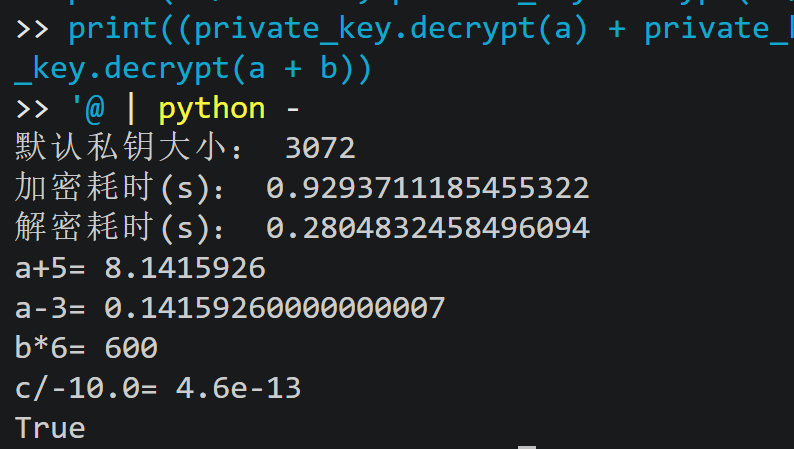
\includegraphics[width=0.95\textwidth]{../src/1.png}
    \caption{Paillier 同态性质验证结果}
\end{figure}

从图中可以看到，程序已经输出了各项运算结果，这与前面的文字分析相对应，说明同态性质验证已经成功完成。

\subsection{隐私信息获取}
在基础实验中，服务器保存一个消息列表，客户端希望只取其中某一项，同时不让服务器知道请求的是哪一项。根据 Paillier 的性质，我们可以设计如下方案：

\begin{framed}
\begin{itemize}
    \item \textbf{服务器端：} 保存消息列表 $data\_list=\{m_1,m_2,\dots,m_n\}$。
    \item \textbf{客户端：}
    \begin{itemize}
        \item 设定目标下标 $pos$；
        \item 构造 one-hot 选择向量 $\{0,\dots,1,\dots,0\}$；
        \item 对其逐位加密，得到 $\{E(0),\dots,E(1),\dots,E(0)\}$；
        \item 将加密后的选择向量发送给服务器。
    \end{itemize}
    \item \textbf{服务器端：}
    \begin{itemize}
        \item 计算
        \[
        c = m_1 \cdot enc\_list[1] + \dots + m_n \cdot enc\_list[n] ;
        \]
        \item 将聚合密文 $c$ 返回给客户端。
    \end{itemize}
    \item \textbf{客户端：} 解密聚合结果，恢复目标消息。
\end{itemize}
\end{framed}

上述协议在工程实现中主要落在“客户端构造加密选择向量”和“服务端完成同态聚合”这两个核心步骤上。对应的关键代码如下：
\begin{lstlisting}[title=基础实验关键代码：选择向量构造与同态聚合,frame=trbl,language={Python}]
def build_selection_vector(public_key, index, size):
    validate_index(index, size)
    return [public_key.encrypt(int(position == index)) for position in range(size)]

def aggregate_query(public_key, plaintexts, selection_vector):
    if len(plaintexts) != len(selection_vector):
        raise ValueError("plaintext dataset and selection vector must have identical length")
    validate_plaintexts(plaintexts, public_key)
    result = public_key.encrypt(0)
    for plaintext, encrypted_selector in zip(plaintexts, selection_vector, strict=True):
        result += encrypted_selector * plaintext
    return result
\end{lstlisting}

这段代码直接对应了实验原理中的 one-hot 查询向量方案。客户端将目标位置编码为“只有一位为 1，其余全为 0”的加密向量；服务端则对每个消息与对应密文选择位做标量乘法并累加。由于只有目标位置的选择位在解密后等于 1，最终聚合结果就只会保留目标消息，从而实现“服务器不知道查的是谁，客户端却能恢复正确消息”的效果。

在真实的 TCP 客户端中，我们还需要把公钥和选择向量序列化后发给服务端，并在收到返回结果后完成解密恢复。对应实现如下：
\begin{lstlisting}[title=基础实验关键代码：客户端查询与结果恢复,frame=trbl,language={Python}]
public_key, private_key = paillier.generate_paillier_keypair(n_length=key_size)
selection_vector = build_selection_vector(public_key, index, dataset_size)
request = {
    "protocol": "pir-lab1",
    "mode": mode,
    "public_key": serialize_public_key(public_key),
    "selection_vector": [serialize_encrypted_number(item) for item in selection_vector],
}

with socket.create_connection((host, port), timeout=30) as sock:
    request_bytes = send_message(sock, request)
    response, response_bytes = recv_message(sock)

result = paillier.EncryptedNumber(
    public_key, int(response["result"]["ciphertext"]), int(response["result"]["exponent"])
)
recovered_value = private_key.decrypt(result)
plaintext = decode_int_to_text(recovered_value)
\end{lstlisting}

这部分代码说明，本实验并不是停留在“数学上可行”的推导，而是已经将 PIR 查询封装为可实际传输的网络请求。客户端本地生成密钥对、构造查询、发送请求并解密返回值，服务端只接触序列化后的公钥和密文选择向量，因此整个实验流程已经具备完整的系统实现形态。

本次实验没有停留在单脚本模拟，而是实现成了真实的 TCP 客户端/服务器结构。首先，我们启动服务端：
\begin{lstlisting}[title=基础实验服务端启动命令,frame=trbl,language={Python}]
python scripts/run_server.py --mode basic --host 127.0.0.1 --port 9101 --count 16
\end{lstlisting}

该命令会在本地开启一个基础版 PIR 服务端，并加载 16 条测试消息，等待客户端发起查询。

然后，我们在客户端发起查询，请求命令如下：
\begin{lstlisting}[title=基础实验客户端查询命令,frame=trbl,language={Python}]
python scripts/run_client.py --mode basic --host 127.0.0.1 --port 9101 --dataset-size 16 --key-size 2048 --index 5
\end{lstlisting}

这里客户端查询的是下标为 5 的消息，同时使用 2048-bit Paillier 密钥来生成加密选择向量。

本次实际运行结果直接见下方截图。结合截图中的服务端日志和客户端输出可以看出，服务端只能看到数据集规模与请求字节数，无法直接恢复目标下标；而客户端最终成功恢复了目标明文 \texttt{record-06|name=Frank|dept=Security|score=85}。同时，本轮实验的请求大小约为 20925 B，响应大小约为 1364 B，说明主要通信开销仍然来自客户端发送的加密选择向量。这说明基础版实验已经实现了“查询位置隐私可被保护、但目标消息仍可正确恢复”的要求。这样，我们就完成了基础版隐私信息获取实验。

\begin{figure}[H]
    \centering
    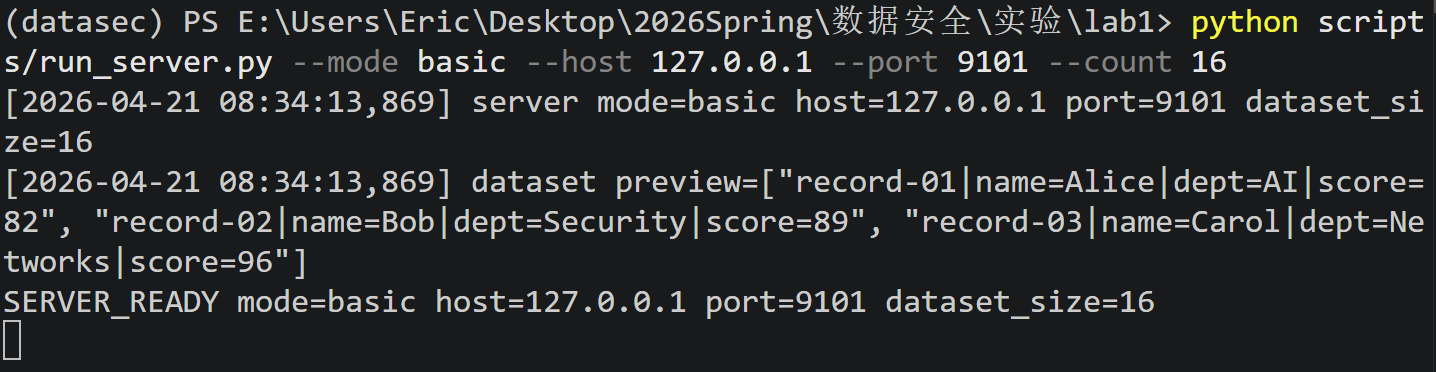
\includegraphics[width=0.95\textwidth]{../src/2.png}
    \caption{基础实验服务端启动并加载数据集}
\end{figure}

这张图展示了服务端启动后的状态，可以看到数据集已经被成功加载，说明基础实验的服务端准备工作已经完成。

\begin{figure}[H]
    \centering
    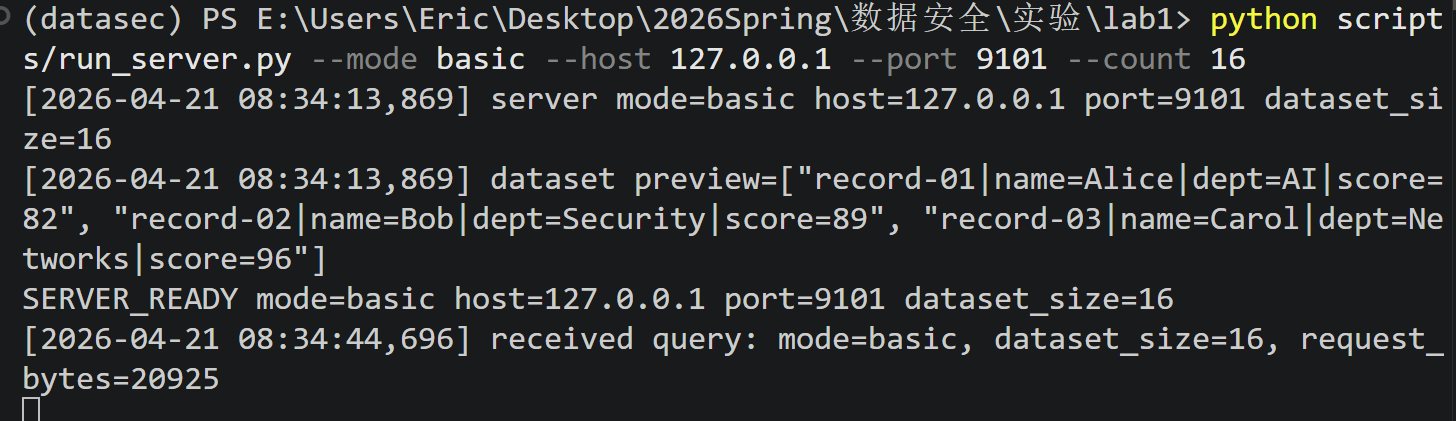
\includegraphics[width=0.95\textwidth]{../src/4.png}
    \caption{基础实验服务端接收加密查询}
\end{figure}

这张图展示了服务端接收到客户端发送的加密选择向量后所记录的日志，可以看到服务端只能观察到查询规模和请求字节数，而无法直接判断目标下标。

\begin{figure}[H]
    \centering
    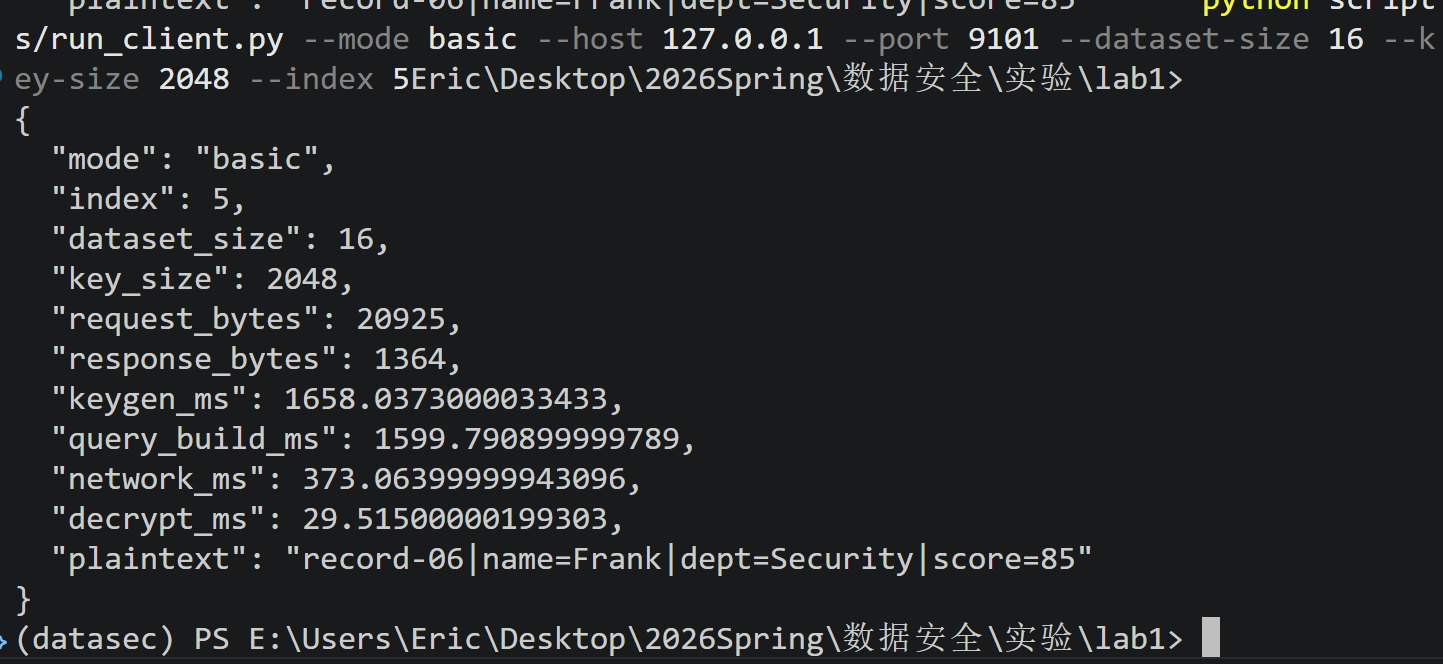
\includegraphics[width=0.95\textwidth]{../src/3.png}
    \caption{基础实验客户端恢复目标明文}
\end{figure}

这张图对应客户端的最终输出结果，可以看到目标明文已经被正确恢复出来。

\subsection{扩展实验探索}
在扩展实验中，服务器不再直接保存明文消息，而是保存经 AES-GCM 加密后的密文包；客户端保存本地 AES 对称密钥。查询阶段仍然使用 Paillier 构造隐私选择向量，服务器返回目标 AES 密文包，我们再在客户端本地完成解密并恢复明文。

与基础实验相比，扩展实验的关键变化不在于 PIR 聚合逻辑本身，而在于“服务器保存什么”。对应的关键代码如下：
\begin{lstlisting}[title=扩展实验关键代码：AES 密文封装与恢复,frame=trbl,language={Python}]
NONCE_SIZE = 12
TAG_SIZE = 16

def encrypt_message(key: bytes, plaintext: str) -> bytes:
    cipher = AES.new(key, AES.MODE_GCM, nonce=get_random_bytes(NONCE_SIZE))
    ciphertext, tag = cipher.encrypt_and_digest(plaintext.encode("utf-8"))
    return cipher.nonce + tag + ciphertext

def decrypt_message(key: bytes, package: bytes) -> str:
    nonce = package[:NONCE_SIZE]
    tag = package[NONCE_SIZE : NONCE_SIZE + TAG_SIZE]
    ciphertext = package[NONCE_SIZE + TAG_SIZE :]
    cipher = AES.new(key, AES.MODE_GCM, nonce=nonce)
    plaintext = cipher.decrypt_and_verify(ciphertext, tag)
    return plaintext.decode("utf-8")
\end{lstlisting}

这段代码的作用是把原始明文记录打包成“随机 \texttt{nonce} + 完整性校验标签 + 密文”的 AES-GCM 数据包。这样一来，服务器端保存的已经不再是明文消息，而是只能在客户端持有正确对称密钥时才能恢复的密文包，从而实现了对静态存储数据的进一步保护。

为了让服务器能够直接对这些密文包执行与基础实验相同的 PIR 聚合，我们还将每条消息预处理为可编码、可聚合的整数表示：
\begin{lstlisting}[title=扩展实验关键代码：构造密文数据集,frame=trbl,language={Python}]
def build_aes_ciphertext_store(messages: list[str], key: bytes) -> list[bytes]:
    if not messages:
        raise ValueError("messages must not be empty")
    return [encrypt_message(key, message) for message in messages]

def build_plaintexts(self) -> list[int]:
    if self.mode == "basic":
        return [encode_text_to_int(message) for message in self.messages]
    if not self.aes_packages:
        raise ValueError("AES ciphertext store is not initialized")
    return [encode_blob_to_int(package) for package in self.aes_packages]
\end{lstlisting}

这里的实现思路很关键：扩展实验并没有改变 Paillier 只能处理整数的事实，而是先把 AES 密文包编码成整数，再沿用基础实验中的同态聚合流程。也就是说，实验的“访问模式保护”仍然由 Paillier PIR 完成，而“服务器静态存储保护”则由 AES-GCM 提供，二者在这里形成了较清晰的组合方案。

首先，我们初始化 AES 密钥：
\begin{lstlisting}[title=AES 密钥初始化命令,frame=trbl,language={Python}]
python scripts/init_aes_key.py demo_aes.key
\end{lstlisting}

这一步会在本地生成一个 AES 对称密钥文件，后续客户端解密和服务端构造密文数据集都要使用该密钥。

然后，我们启动扩展实验服务端：
\begin{lstlisting}[title=扩展实验服务端启动命令,frame=trbl,language={Python}]
python scripts/run_server.py --mode aes --host 127.0.0.1 --port 9102 --count 16 --key-file demo_aes.key
\end{lstlisting}

最后，我们在客户端发起扩展查询：
\begin{lstlisting}[title=扩展实验客户端查询命令,frame=trbl,language={Python}]
python scripts/run_client.py --mode aes --host 127.0.0.1 --port 9102 --dataset-size 16 --key-size 2048 --index 5 --key-file demo_aes.key
\end{lstlisting}

本次实际运行结果同样直接见下方截图。由截图可见，AES 密钥已经成功初始化，服务端能够在 \texttt{mode=aes} 模式下正常接收查询，客户端最终也恢复出了目标明文。结合客户端截图中的结果字段可以看到，本轮扩展实验的请求大小约为 20922 B，响应大小约为 1372 B，客户端本地解密耗时约为 47.49 ms。相比基础实验，扩展实验进一步实现了服务端静态存储密文，而最终明文恢复仅在客户端本地完成。这样，我们就完成了扩展实验的验证。

\begin{figure}[H]
    \centering
    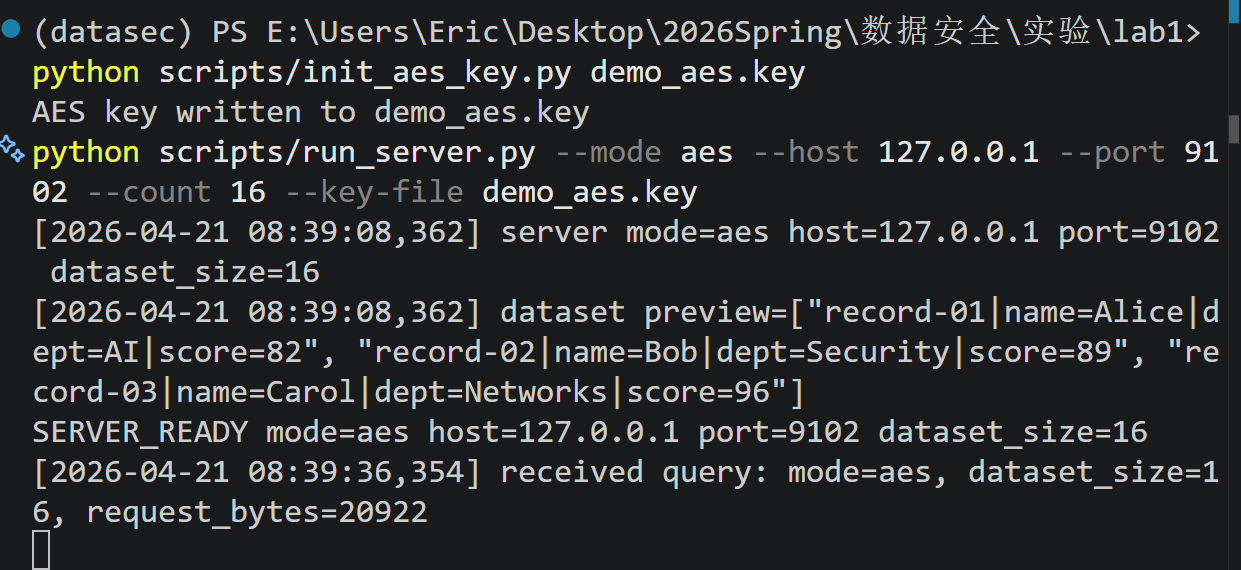
\includegraphics[width=0.95\textwidth]{../src/8.png}
    \caption{扩展实验 AES 密钥初始化与服务端处理查询}
\end{figure}

这张图展示了扩展实验中 AES 密钥初始化成功以及服务端接收查询后的处理状态，说明密文数据集已经能够配合 PIR 查询流程正常运行。

\begin{figure}[H]
    \centering
    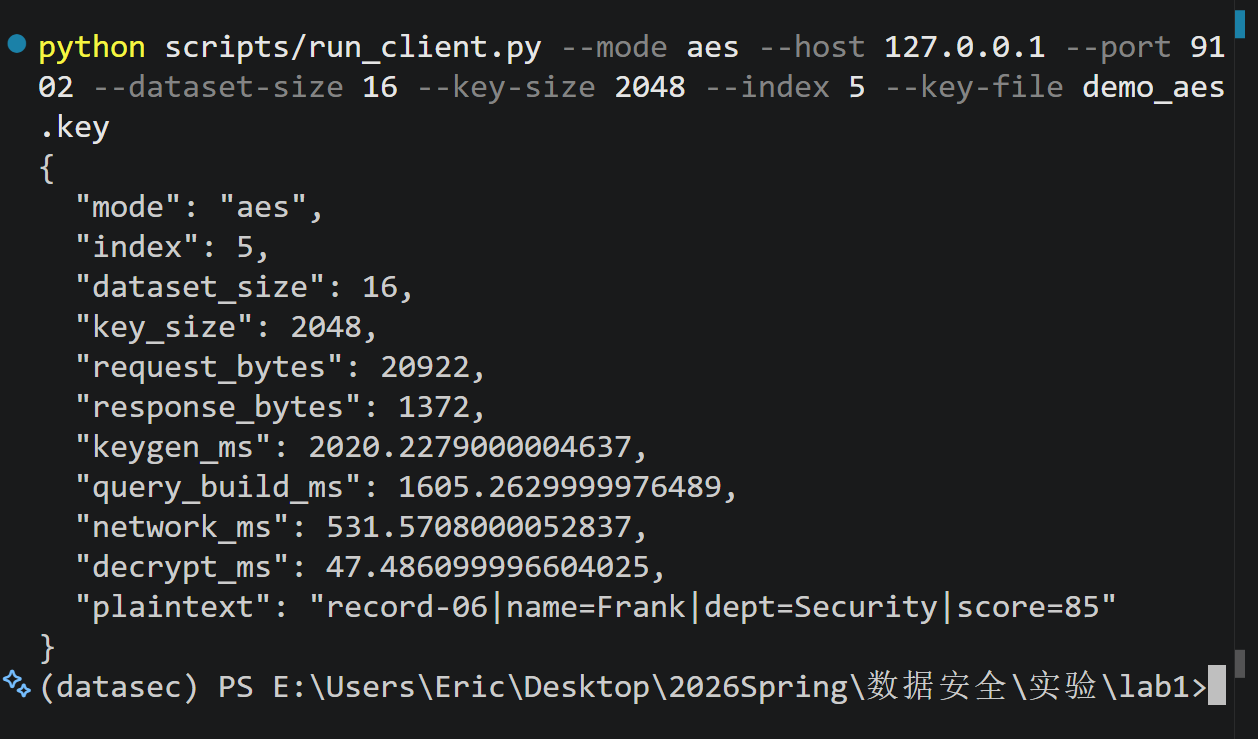
\includegraphics[width=0.95\textwidth]{../src/7.png}
    \caption{扩展实验客户端恢复目标明文}
\end{figure}

这张图对应扩展实验客户端的输出结果，可以看到客户端在取回目标密文包后，已经进一步完成本地解密并恢复出正确明文。

\subsection{性能测试与结果分析}
为了使本次报告在实验展示上更加完整，我们补充了系统化基准测试（benchmark），对消息规模、密钥长度以及基础版/扩展版的开销进行统计。运行命令如下：
\begin{lstlisting}[title=基准测试运行命令,frame=trbl,language={Python}]
python scripts/benchmark.py
\end{lstlisting}

消息规模测试结果如表 \ref{tab:dataset-scale} 所示。
\begin{table}[H]
    \centering
    \resizebox{\textwidth}{!}{
    \begin{tabular}{ccccc}
    \toprule
    $m$ & 平均总耗时/ms & 平均请求字节/B & 平均响应字节/B & 说明 \\
    \midrule
    8  & 1845.71 & 10811.33 & 1363.00 & 请求向量较短，整体耗时最低 \\
    16 & 2699.26 & 20920.67 & 1364.00 & 请求大小随消息规模继续增长 \\
    32 & 4678.05 & 41142.67 & 1364.00 & 查询构造与网络传输继续增加 \\
    64 & 8769.53 & 81588.00 & 1363.67 & 请求体积约为 $m=8$ 时的 7.55 倍 \\
    \bottomrule
    \end{tabular}}
    \caption{消息规模对性能与通信量的影响（2048-bit，基础实验）}
    \label{tab:dataset-scale}
\end{table}

密钥长度测试结果如表 \ref{tab:key-scale} 所示。
\begin{table}[H]
    \centering
    \resizebox{\textwidth}{!}{
    \begin{tabular}{ccccc}
    \toprule
    密钥长度/bit & 平均总耗时/ms & 平均请求字节/B & 平均响应字节/B & 说明 \\
    \midrule
    1024 & 454.14  & 10748.33 & 747.33  & 运行最快，但安全裕度较低 \\
    2048 & 2590.74 & 20921.67 & 1363.67 & 兼顾安全性与可演示性 \\
    3072 & 9100.20 & 31090.67 & 1979.67 & 计算与通信开销显著上升 \\
    \bottomrule
    \end{tabular}}
    \caption{Paillier 密钥长度对性能与通信量的影响（基础实验，$m=16$）}
    \label{tab:key-scale}
\end{table}

基础版与扩展版的开销对比如表 \ref{tab:mode-compare} 所示。
\begin{table}[H]
    \centering
    \resizebox{\textwidth}{!}{
    \begin{tabular}{ccccc}
    \toprule
    模式 & 平均总耗时/ms & 平均请求字节/B & 平均响应字节/B & 平均解密耗时/ms \\
    \midrule
    basic & 2622.82 & 20923.00 & 1363.33 & 27.37 \\
    aes   & 2418.77 & 20917.33 & 1372.00 & 28.13 \\
    \bottomrule
    \end{tabular}}
    \caption{基础版与扩展版对比（$m=16$，2048-bit）}
    \label{tab:mode-compare}
\end{table}

实验结果说明：
\begin{itemize}
    \item 当 $m$ 从 8 增长到 64 时，请求大小从 10811.33 B 增至 81588.00 B，而响应始终约为 1364 B，说明主要通信开销来自客户端发送的加密选择向量；
    \item 密钥长度增大后，密钥生成、查询构造和同态聚合成本同步上升；3072-bit 相比 2048-bit 的总耗时约提升到 3.5 倍，通信量也明显变大；
    \item 本轮本地 benchmark 中 \texttt{aes} 的平均总耗时略低于 \texttt{basic}，但两者处于同一数量级。这一差异更适合视为本机多轮测试波动，而不是“AES 模式天然更快”；更稳妥的结论是扩展模式增加了响应密文包大小，并引入了客户端本地 AES-GCM 解密步骤。
\end{itemize}

此外，我们还通过 \texttt{pytest} 完成了自动化验证：
\begin{figure}[H]
    \centering
    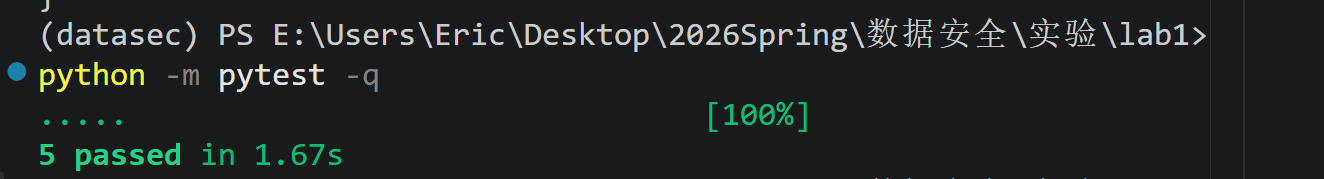
\includegraphics[width=0.78\textwidth]{../src/9.png}
    \caption{自动化测试全部通过}
\end{figure}

这张图说明自动化测试已经全部通过，从侧面验证了基础版与扩展版核心功能在当前实现下都能够稳定运行。
综合以上表格与测试结果可以看出，2048-bit 配置在安全性、通信量和运行开销之间取得了较好的平衡；扩展模式虽然引入了额外的本地解密步骤，但在保持查询隐私的同时进一步提升了服务器静态存储数据的保护能力。

\section{实验心得与体会}
本次实验在课程要求的基础上完成了较完整的工程化实现。整体方法与课件中基于 Paillier 的 one-hot PIR 思路一致，但在实现层面我们进一步扩展为真实的客户端/服务器结构，并补充了协议序列化、自动化测试和基准测试分析，使整个实验更接近一个可复现的小型系统。

在实验过程中，我们对 Paillier 半同态加密的理解更加清晰：它并不适合做任意运算，但非常适合用于构造 one-hot 查询向量和聚合结果，这一点恰好对应了隐私信息获取问题的需求。同时，扩展实验也让我们进一步理解了“存储保护”和“访问模式保护”可以通过对称加密与同态加密的组合来共同实现。

总体来看，我们不仅完成了题目要求，也对同态加密的适用边界、实现约束以及工程化落地方式有了更直接的认识。本次报告中的日志、截图、测试和基准测试数据均来自我们在 2026 年 4 月 21 日的实际运行结果。若继续扩展，我们还可以进一步尝试恶意安全模型、多服务器 PIR 或者更高效的通信压缩方案，以提升系统的实际应用价值。这样，我们也就把课件中的 Paillier PIR 思路落实成了一套可以直接演示和复现的实验流程。

\end{document}
